\documentclass{article}

\usepackage[a4paper, margin=2cm]{geometry}
\usepackage[utf8]{inputenc}

\usepackage[czech]{babel}
\usepackage{fvextra}
\usepackage{csquotes}
\usepackage{parskip}

\usepackage{float}
\usepackage{amsmath}
\usepackage{textcomp}
\usepackage{gensymb}
\usepackage{graphicx}
\graphicspath{{images}}

\usepackage[hidelinks, unicode, pdfusetitle]{hyperref}

\usepackage{mathtools}
\DeclarePairedDelimiter\ceil{\lceil}{\rceil}
\DeclarePairedDelimiter\floor{\lfloor}{\rfloor}

\title{34-4-4 Geometrie}
\author{Benjamin Swart}

\setcounter{secnumdepth}{1}

\begin{document}

\maketitle

\section{Prvotní pozorování}
\label{intro}

Počet kusů, které řezem vzniknou, je rovný polovině počtu protnutých stran plus jedna. Každý jednotlivý \enquote{podřez} totiž začíná a končí stranou a dělí jeden kus na dva. Na začátku máme kus jeden.

Bez ztráty na obecnosti můžeme předpokládat, že se naše přímka bude dotýkat\footnote{Dotek přímky \(p\) bodu \(B\) budeme definovat tak, že \(|pB| = \epsilon\), neboli že přímka vede \enquote{těsně vedle} bodu.} dvou vrcholů. Pokud je optimálním řešením přímka, které se dvou vrcholů nedotýká, tak jí můžeme posouvat po kolmici k ní, tokud se nebude dotýkat jednoho bodu, a následně otáčet kolem prvního bodu, dokud se nebude dotýkat druhého. Jelikož naším posouváním nepřekročíme žádný bod, tak se zajisté nezbavíme žádného protnutí úsečky.

\section{Algoritmus pro přímku rovnoběžnou s osou x}

Použijeme zametání roviny. Z bodů poskládáme seznam úseček. Horní (největší \(y\)) bod úsečky prohlásíme za její začátek a dolní za její konec. Tyto body následně seřadíme podle souřadnice \(y\). Nakonec si uložíme do \(m\) číslo \(0\), a začneme procházet seznam. Když narazíme na začátek úsečky, tak k \(m\) přičteme \(1\), a když narazíme na konec tak \(1\) odečteme. Řešení bude nejvyšší hodnota, které \(m\) nabude (děleno dvěmi, plus jedna).

Tento algoritmus běží v \(O(n*log(n))\).

\section{Obecný algoritmus}

Jelikož jsme v sekci \ref{intro} dokázali, že se přímka bude dotýkat dvou bodů, tak nám stačí co nejrychleji projít všechny možné takové přímky a určit, kolik protnou úseček.

Projdeme všechny vrcholy \(O\) a z každého spustíme \enquote{ometání roviny}. Ometáním roviny projdeme všechny přímky, které bodem \(O\) prochází. Jelikož není vhodné, aby přímka vrcholem přímo procházela, tak bod o posuneme mírně směrem dovnitř tupého úhlu, který se stranami svírá. Tím získáme možnost tento úhel protnout.

Všechny vrcholy označíme úhlem, který svírá přímka vedená do nich z bodu \(O\) s osou \(x\). Jelikož přímka vede z bodu \(O\) dvěmi směry, jedním do každé poloroviny, tak budou tyto úhly nejvýše \(180\degree\).

\begin{figure}[H]
    \centering
    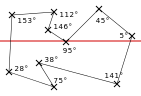
\includegraphics[scale=0.5]{swipe001.pdf}
\end{figure}

Poté postupujeme podobně jako u zametání roviny. Vytvoříme si seřazený seznam hranic stran označených jako začátek nebo konec.

Jako počáteční stav si uložíme počet stran, kterou protíná počáteční přímka rovnoběžná s osou \(x\). Toho docílíme lineárním průchodem seznamu, kdy pro každou stranu kontrolujeme, zda naši přímku protíná.

Poté opět procházíme seznam a přičítáme a odčítáme \(1\) k/od počtu úseček.

\begin{figure}[H]
    \centering
    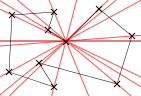
\includegraphics[scale=0.5]{swipe002.pdf}
\end{figure}

Uložíme si maximální počet úseček, na který za celý běh algoritmu narazíme. Nakonec ho vydělíme dvěmi a přičteme jedna, čímž získáme řešení.

Tento algoritmus \(n\)-krát seřadí seznam s \(n\) prvky. Běží tedy v \(O(n^2*log(n))\). Paměti potřebuje \(O(n)\).

\end{document}
